% Options for packages loaded elsewhere
\PassOptionsToPackage{unicode}{hyperref}
\PassOptionsToPackage{hyphens}{url}
%
\documentclass[
  11pt,
]{article}
\usepackage{amsmath,amssymb}
\usepackage{iftex}
\ifPDFTeX
  \usepackage[T1]{fontenc}
  \usepackage[utf8]{inputenc}
  \usepackage{textcomp} % provide euro and other symbols
\else % if luatex or xetex
  \usepackage{unicode-math} % this also loads fontspec
  \defaultfontfeatures{Scale=MatchLowercase}
  \defaultfontfeatures[\rmfamily]{Ligatures=TeX,Scale=1}
\fi
\usepackage{lmodern}
\ifPDFTeX\else
  % xetex/luatex font selection
\fi
% Use upquote if available, for straight quotes in verbatim environments
\IfFileExists{upquote.sty}{\usepackage{upquote}}{}
\IfFileExists{microtype.sty}{% use microtype if available
  \usepackage[]{microtype}
  \UseMicrotypeSet[protrusion]{basicmath} % disable protrusion for tt fonts
}{}
\makeatletter
\@ifundefined{KOMAClassName}{% if non-KOMA class
  \IfFileExists{parskip.sty}{%
    \usepackage{parskip}
  }{% else
    \setlength{\parindent}{0pt}
    \setlength{\parskip}{6pt plus 2pt minus 1pt}}
}{% if KOMA class
  \KOMAoptions{parskip=half}}
\makeatother
\usepackage{xcolor}
\usepackage[margin=0.5in]{geometry}
\usepackage{longtable,booktabs,array}
\usepackage{calc} % for calculating minipage widths
% Correct order of tables after \paragraph or \subparagraph
\usepackage{etoolbox}
\makeatletter
\patchcmd\longtable{\par}{\if@noskipsec\mbox{}\fi\par}{}{}
\makeatother
% Allow footnotes in longtable head/foot
\IfFileExists{footnotehyper.sty}{\usepackage{footnotehyper}}{\usepackage{footnote}}
\makesavenoteenv{longtable}
\usepackage{graphicx}
\makeatletter
\def\maxwidth{\ifdim\Gin@nat@width>\linewidth\linewidth\else\Gin@nat@width\fi}
\def\maxheight{\ifdim\Gin@nat@height>\textheight\textheight\else\Gin@nat@height\fi}
\makeatother
% Scale images if necessary, so that they will not overflow the page
% margins by default, and it is still possible to overwrite the defaults
% using explicit options in \includegraphics[width, height, ...]{}
\setkeys{Gin}{width=\maxwidth,height=\maxheight,keepaspectratio}
% Set default figure placement to htbp
\makeatletter
\def\fps@figure{htbp}
\makeatother
\setlength{\emergencystretch}{3em} % prevent overfull lines
\providecommand{\tightlist}{%
  \setlength{\itemsep}{0pt}\setlength{\parskip}{0pt}}
\setcounter{secnumdepth}{-\maxdimen} % remove section numbering
% definitions for citeproc citations
\NewDocumentCommand\citeproctext{}{}
\NewDocumentCommand\citeproc{mm}{%
  \begingroup\def\citeproctext{#2}\cite{#1}\endgroup}
\makeatletter
 % allow citations to break across lines
 \let\@cite@ofmt\@firstofone
 % avoid brackets around text for \cite:
 \def\@biblabel#1{}
 \def\@cite#1#2{{#1\if@tempswa , #2\fi}}
\makeatother
\newlength{\cslhangindent}
\setlength{\cslhangindent}{1.5em}
\newlength{\csllabelwidth}
\setlength{\csllabelwidth}{3em}
\newenvironment{CSLReferences}[2] % #1 hanging-indent, #2 entry-spacing
 {\begin{list}{}{%
  \setlength{\itemindent}{0pt}
  \setlength{\leftmargin}{0pt}
  \setlength{\parsep}{0pt}
  % turn on hanging indent if param 1 is 1
  \ifodd #1
   \setlength{\leftmargin}{\cslhangindent}
   \setlength{\itemindent}{-1\cslhangindent}
  \fi
  % set entry spacing
  \setlength{\itemsep}{#2\baselineskip}}}
 {\end{list}}
\usepackage{calc}
\newcommand{\CSLBlock}[1]{\hfill\break#1\hfill\break}
\newcommand{\CSLLeftMargin}[1]{\parbox[t]{\csllabelwidth}{\strut#1\strut}}
\newcommand{\CSLRightInline}[1]{\parbox[t]{\linewidth - \csllabelwidth}{\strut#1\strut}}
\newcommand{\CSLIndent}[1]{\hspace{\cslhangindent}#1}
\newenvironment{cols}[1][]{}{}

\newenvironment{col}[1]{\begin{minipage}{#1}\ignorespaces}{%
\end{minipage}
\ifhmode\unskip\fi
\aftergroup\useignorespacesandallpars}

\def\useignorespacesandallpars#1\ignorespaces\fi{%
#1\fi\ignorespacesandallpars}

\makeatletter
\def\ignorespacesandallpars{%
  \@ifnextchar\par
    {\expandafter\ignorespacesandallpars\@gobble}%
    {}%
}
\makeatother
\usepackage{hyperref}
\usepackage{array}
\usepackage{caption}
\usepackage{graphicx}
\usepackage{multirow}
\usepackage{hhline}
\usepackage{calc}
\usepackage{tabularx}
\usepackage[para,online,flushleft]{threeparttable}
\DeclareMathOperator{\logit}{logit}
\DeclareMathOperator{\var}{var}
\ifLuaTeX
  \usepackage{selnolig}  % disable illegal ligatures
\fi
\IfFileExists{bookmark.sty}{\usepackage{bookmark}}{\usepackage{hyperref}}
\IfFileExists{xurl.sty}{\usepackage{xurl}}{} % add URL line breaks if available
\urlstyle{same}
\hypersetup{
  pdftitle={Analysis of Health Survey for England (HSE) 2019},
  pdfauthor={Candidate Numbers Here},
  hidelinks,
  pdfcreator={LaTeX via pandoc}}

\title{Analysis of Health Survey for England (HSE) 2019}
\author{Candidate Numbers Here}
\date{March 08, 2024}

\begin{document}
\maketitle
\begin{abstract}
This report provides an analysis of data related to health, age,
socio-economic factors and lifestyle habits in adults (from the age of
16) from the population in England, derived from the Health Survey for
England 2019.
\end{abstract}

\pagenumbering{gobble}

\newpage

\subsection{Summary (Non-Technical)}\label{summary-non-technical}

\subsection{Introduction}\label{introduction}

In the UK, smoking, vaping, and alcohol consumption are widespread,
particularly among youngsters. It is crucial to be aware of the
consequences and dangers of these habits, and the complications they can
cause in later-life. The Office for National Statistics (ONS), regarded
as the foremost statistical institute in the UK, is the ``go-to'' for
insights into public health trends. According to their estimations,
approximately 14.1\% of the adult population aged 18 and above were
identified as cigarette smokers (\citeproc{ref-1ONS}{ONS 2019a}).
Furthermore, their data revealed there were 7,565 deaths attributed to
alcohol-specific causes in 2019 (\citeproc{ref-2ONS}{ONS 2019b}). These
statistics alone warrant a need for an understanding of health-related
behaviours and the outcome. Therefore, the aim of our study is to
investigate not only the prevalence but also the severity of these
habits, exploring different socioeconomic factors that may potentially
contribute to each. Additionally, we will investigate the greater
implications of these bad habits and how they relate to systolic blood
pressure levels throughout the UK population.

\subsection{Exploratory Analysis}\label{exploratory-analysis}

\textbf{We start by investigating the data}

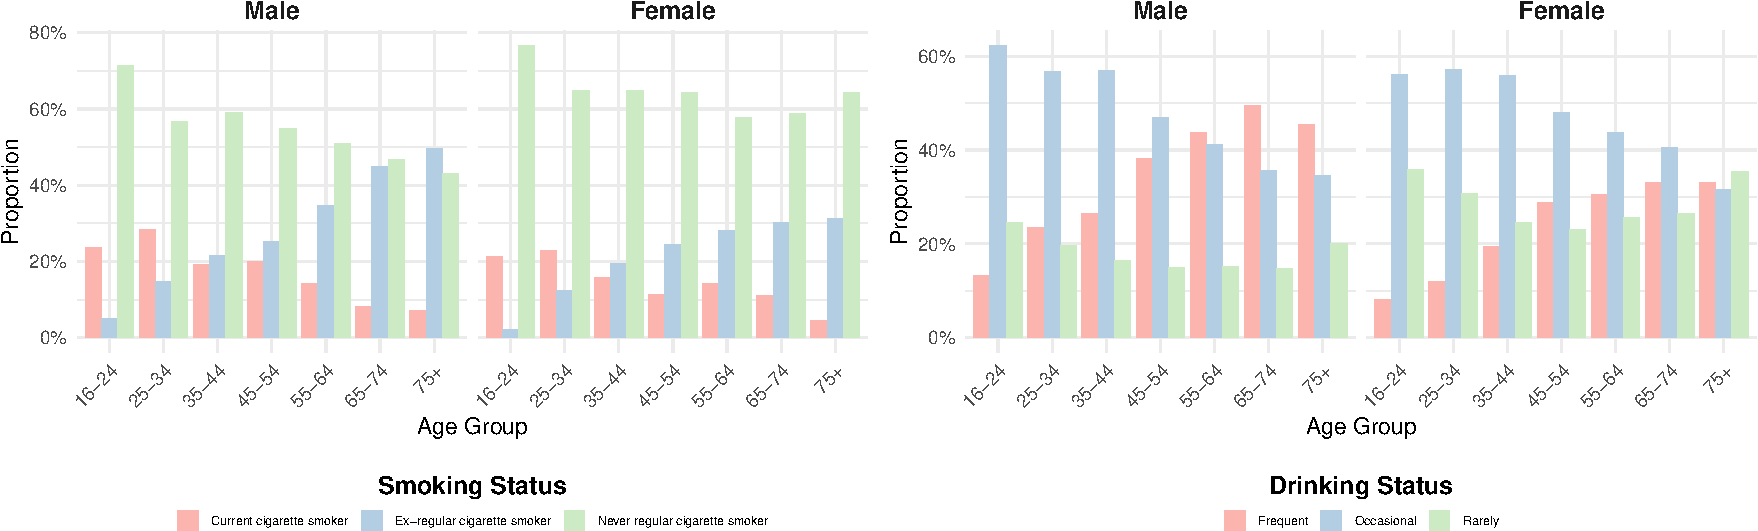
\includegraphics{Coursework_files/figure-latex/output smoking and drinking by age plot-1.pdf}
\\

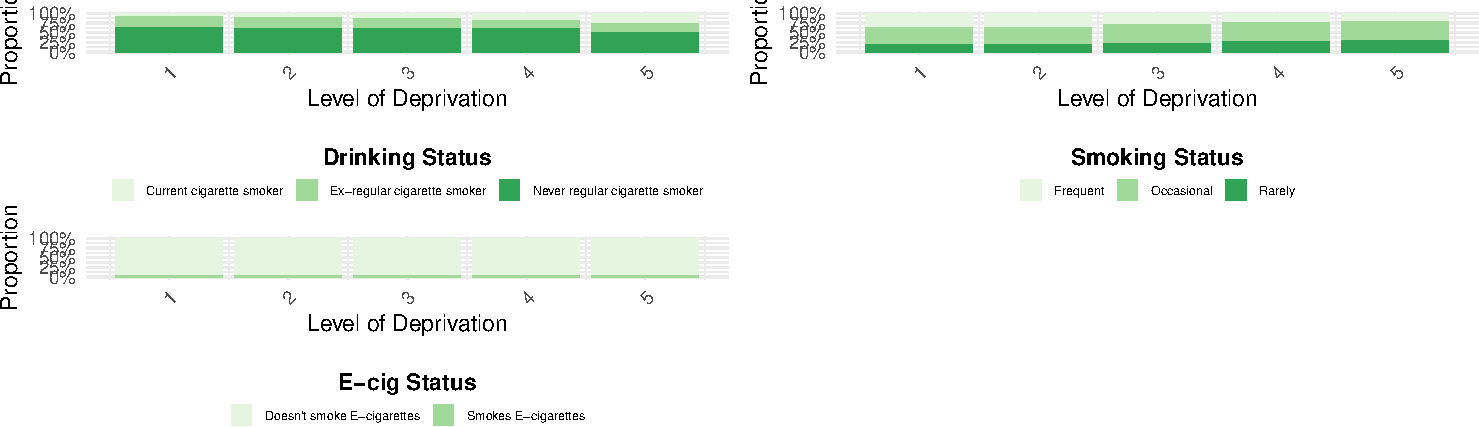
\includegraphics{Coursework_files/figure-latex/output deprivation plot-1.pdf}\\

\subsection{Methology}\label{methology}

\textbf{Define all variables used in analysis}

\subsection{Analysis}\label{analysis}

\subsubsection{What is the prevelance of drinking, smoking and E-cig
usage?}\label{what-is-the-prevelance-of-drinking-smoking-and-e-cig-usage}

To calculate the prevalence of each habit we assume each of the \(n\)
observations, \(x_1,…,x_n\) , to be independent, identically distributed
(iid) random variables (RVs) where
\(x_i \sim Bern(p)\, \forall i=1,…,n\) and \(p\) denotes the probability
of an observation having the relevant habit. We use the household
weights to calculate a weighted Maximum Likelihood Estimate (MLE) of
\(p\). That is, letting \(w_i\) denote the weight of the \(i^{th}\)
observation, we alter the standard likelihood function of a Bernoulli
distribution as below:
\[L(p|\textbf{x}) = \prod_{i = 1}^{n} (p^{x_i}(1-p)^{1-x_i})^{w_i}\]
From this, we calculate our weighted MLE as:
\[\widehat{p} = \frac{\sum_{i=1}^{n} x_iw_i}{\sum_{i=1}^{n} w_i}\]

It can also be shown that this MLE has variance given by
\(\mathop{\mathrm{var}}(\widehat{p})=\frac{p(1-p)}{\sum_{i=1}^{n}w_i}\),
which we can estimate using \(\widehat{p}\) and use large sample
properties of the MLE to get a normal approximation and estimate 95\%
confidence intervals for each habit, which are shown in the table below.

\begin{longtable}[]{@{}lll@{}}
\caption{Estimates and 95\% Confidence Intervals for \% of
Population}\tabularnewline
\toprule\noalign{}
Category & Estimate & C.I. \\
\midrule\noalign{}
\endfirsthead
\toprule\noalign{}
Category & Estimate & C.I. \\
\midrule\noalign{}
\endhead
\bottomrule\noalign{}
\endlastfoot
Drinking & 80.3\% & (79.5\%, 81.2\%) \\
Smoking & 16.5\% & (15.7\%, 17.3\%) \\
Smoking E-cigarettes & 4.28\% & (3.84\%, 4.72\%) \\
\end{longtable}

\textbf{Interpretation of table/results - e-cig is much lower, drinking
very common etc}

\textbf{We can also\ldots{}}

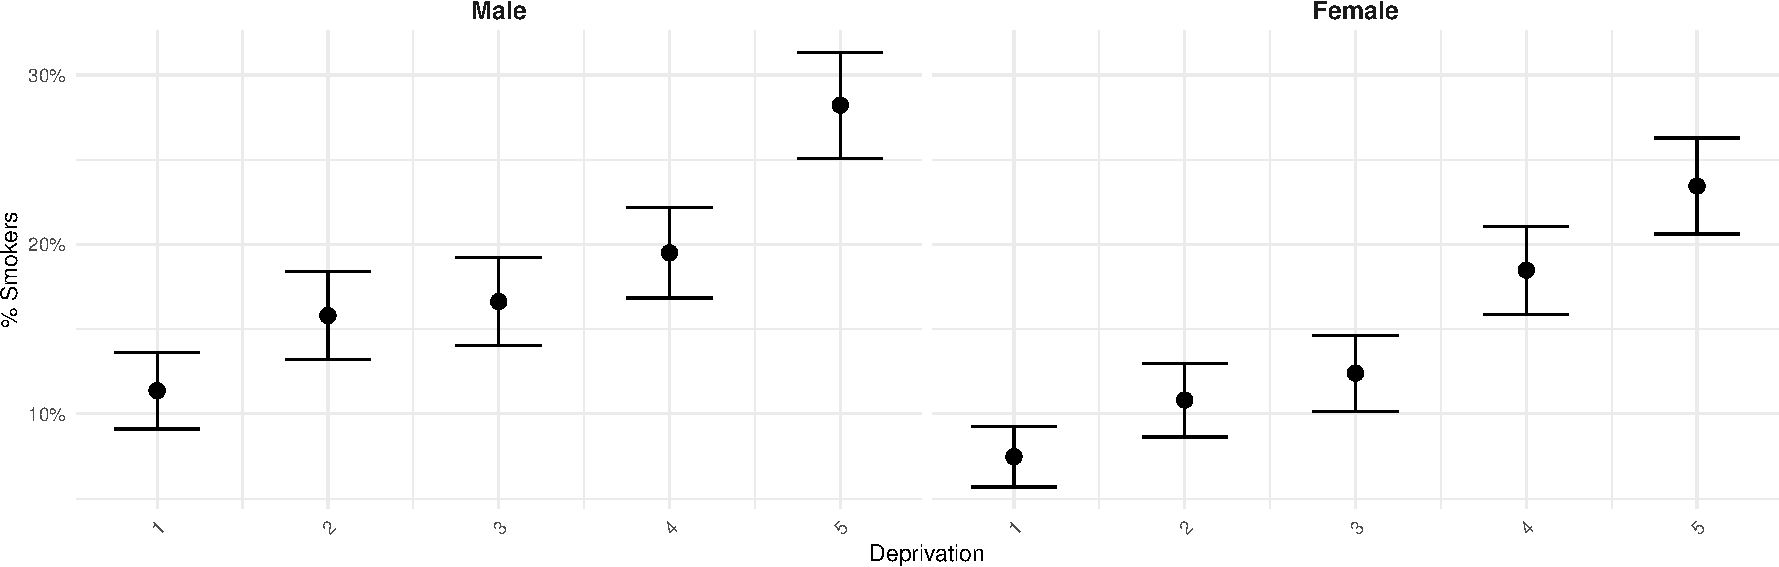
\includegraphics{Coursework_files/figure-latex/output prevelance plot-1.pdf}\\

\subsubsection{How is smoking associated with socioeconomic factors and
age?}\label{how-is-smoking-associated-with-socioeconomic-factors-and-age}

\textbf{Explanation of why we split into test/train dataset.}

This leaves us with 6563 observations in our training dataset. The
number of missing observations for each are shown:

\begin{longtable}[]{@{}lrl@{}}
\caption{Missing values in the training dataset}\tabularnewline
\toprule\noalign{}
Variable & Missing Values & \% Missing \\
\midrule\noalign{}
\endfirsthead
\toprule\noalign{}
Variable & Missing Values & \% Missing \\
\midrule\noalign{}
\endhead
\bottomrule\noalign{}
\endlastfoot
omsysval & 3250 & 49.5\% \\
BMIVal & 1225 & 18.7\% \\
dnoft\_19 & 1203 & 18.3\% \\
cigdyal\_19 & 47 & 0.716\% \\
cigsta3\_19 & 45 & 0.686\% \\
NDPNow\_19 & 41 & 0.625\% \\
d7many3\_19 & 41 & 0.625\% \\
drinkYN\_19 & 40 & 0.609\% \\
topqual2 & 36 & 0.549\% \\
origin2 & 24 & 0.366\% \\
marstatD & 1 & 0.0152\% \\
\end{longtable}

\textbf{Explanation of first model - binomial with logit link}

\begin{longtable}[]{@{}
  >{\raggedright\arraybackslash}p{(\columnwidth - 10\tabcolsep) * \real{0.5940}}
  >{\raggedleft\arraybackslash}p{(\columnwidth - 10\tabcolsep) * \real{0.0752}}
  >{\raggedleft\arraybackslash}p{(\columnwidth - 10\tabcolsep) * \real{0.0677}}
  >{\raggedleft\arraybackslash}p{(\columnwidth - 10\tabcolsep) * \real{0.0827}}
  >{\raggedleft\arraybackslash}p{(\columnwidth - 10\tabcolsep) * \real{0.0752}}
  >{\raggedleft\arraybackslash}p{(\columnwidth - 10\tabcolsep) * \real{0.1053}}@{}}
\caption{Comparison of selected model evaluations}\tabularnewline
\toprule\noalign{}
\begin{minipage}[b]{\linewidth}\raggedright
Linear Predictor
\end{minipage} & \begin{minipage}[b]{\linewidth}\raggedleft
Train AIC
\end{minipage} & \begin{minipage}[b]{\linewidth}\raggedleft
Test AUC
\end{minipage} & \begin{minipage}[b]{\linewidth}\raggedleft
Train RMSE
\end{minipage} & \begin{minipage}[b]{\linewidth}\raggedleft
Test RMSE
\end{minipage} & \begin{minipage}[b]{\linewidth}\raggedleft
Test Accuracy
\end{minipage} \\
\midrule\noalign{}
\endfirsthead
\toprule\noalign{}
\begin{minipage}[b]{\linewidth}\raggedright
Linear Predictor
\end{minipage} & \begin{minipage}[b]{\linewidth}\raggedleft
Train AIC
\end{minipage} & \begin{minipage}[b]{\linewidth}\raggedleft
Test AUC
\end{minipage} & \begin{minipage}[b]{\linewidth}\raggedleft
Train RMSE
\end{minipage} & \begin{minipage}[b]{\linewidth}\raggedleft
Test RMSE
\end{minipage} & \begin{minipage}[b]{\linewidth}\raggedleft
Test Accuracy
\end{minipage} \\
\midrule\noalign{}
\endhead
\bottomrule\noalign{}
\endlastfoot
\(\mathop{\mathrm{logit}}(\mu_i) \sim a_i + a_i^2 + m_i + q_i + u_i + o_i + t_i + s_i + q_i:u_i\)
& 4828.4 & 0.738 & 0.335 & 0.352 & 0.836 \\
\(\mathop{\mathrm{logit}}(\mu_i) \sim a_i + a_i^2 + m_i + q_i + u_i + o_i + t_i + s_i\)
& 4828.8 & 0.739 & 0.335 & 0.352 & 0.836 \\
\(\mathop{\mathrm{logit}}(\mu_i) \sim a_i + m_i + q_i + u_i + o_i + t_i + s_i\)
& 4875.4 & 0.724 & 0.336 & 0.355 & 0.832 \\
\(\mathop{\mathrm{logit}}(\mu_i) \sim a_i^{(5)} + m_i + q_i + u_i + o_i + t_i + s_i\)
& 4843.6 & 0.741 & 0.335 & 0.352 & 0.839 \\
\(\mathop{\mathrm{logit}}(\mu_i) \sim a_i^{(10)} + m_i + q_i + u_i + o_i + t_i + s_i\)
& 4848.8 & 0.735 & 0.335 & 0.352 & 0.837 \\
\end{longtable}

\textbf{Explain why we selected the model we did - lowest AIC}

\textbf{Some model diagnostics}

\begin{figure}
\centering
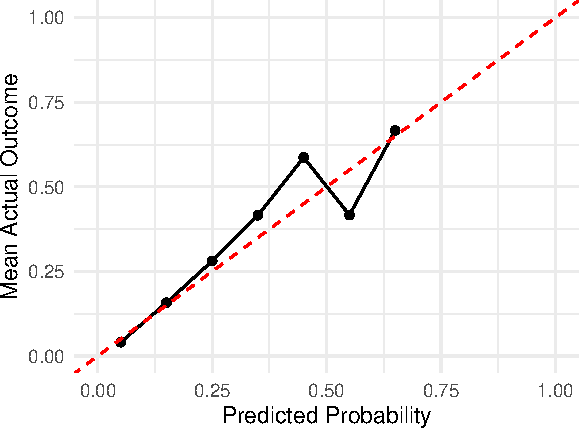
\includegraphics{Coursework_files/figure-latex/output calibration chart-1.pdf}
\caption{Calibration chart for binomial model}
\end{figure}

\textbf{Interpretation of model coefficients etc}

\textbf{Limitations of model}

\subsubsection{Which lifestyle habits are associated with systolic blood
pressure?}\label{which-lifestyle-habits-are-associated-with-systolic-blood-pressure}

\textbf{Question Three}

\subsection{Results/Conclusion}\label{resultsconclusion}

\newpage

\section*{References}\label{references}
\addcontentsline{toc}{section}{References}

\phantomsection\label{refs}
\begin{CSLReferences}{1}{0}
\bibitem[\citeproctext]{ref-1ONS}
ONS. 2019a. {``{Adult smoking habits in the UK: 2019}.''}
\url{https://shorturl.at/qQW27}.

\bibitem[\citeproctext]{ref-2ONS}
---------. 2019b. {``{Alcohol-specific deaths in the UK: registered in
2019}.''} \url{https://shorturl.at/gqxY1}.

\end{CSLReferences}

\end{document}
